\chapter{Generación de trayectorias}\label{cap:gen_tray}

En el apartado anterior se ha diseñado un controlador cuyo objetivo es seguir una trayectoria deseada minimizando el error de seguimiento. En este apartado se tratará sobre la forma en la que se generan estas trayectorias. Este desarrollo se realiza entorno a una trayectoria unidimensional en un único eje de desplazamiento , el eje $x$. Este desarrollo es ampliable al espacio tridimensional realizando una trayectoria por cada eje.


\section{Trayectorias óptimas}\label{trajectoriasoptimas:cap}
El objetivo general del control óptimo es encontrar la función $x^*(t)$ que minimiza la expresión
\begin{equation}
	x^*(t) =  \underset{x(t)}{argmin}\int_{0}^{T}\mathcal{L}\left(x^{(n)},x^{(n-1)},...,\dot{x},x,t\right)\, dt
\end{equation}
siendo $\mathcal{L}$ el índice que se debe optimizar.

Cuando el objetivo es generar trayectorias suaves la forma de la expresión a optimizar es :
\begin{equation}
	x^*(t) = \underset{x(t)}{argmin}\int_{0}^{T}\left(x^{(n)}\right)^2\, dt
\end{equation}
siendo $x^{(n)} = u $, la magnitud de control que se desea minimizar. El valor del parámetro $n\in\mathbb{N}$, expresa el grado de la derivada de la acción de control $u$, es decir, para generar trayectorias de mínima distancia, se empleará un valor de $n=1$, por lo que $u = \dot{x}$, mientras que para generar trayectorias de mínima sobreacceleración (\textit{jerk}) se empleará un valor de $n=3$, por lo que $u = \dddot{x}$.

De forma general la expresión a optimizar será:
	\begin{equation}
		x^*(t) = \underset{x(t)}{argmin}\int_{0}^{T}\mathcal{L}\left(x^{(n)}, x^{(n-1)},...,\dot{x},x,t\right)\, dt
	\end{equation}

De la  ecuación de Euler-Lagrange se obtiene que la la función ófptima $x^*(t)$ debe satisfacer:
\begin{equation}
	\frac{\partial\mathcal{L}}{\partial x} + \sum_{i=1}^{n}(-1)^i \frac{d^i}{dt^i}\left(\frac{\partial\mathcal{L}}{\partial x^i}\right)  = 0
\end{equation}
Si particularizamos la expresión anterior a expresiones donde $\mathcal{L} =\left(x^{(n)}\right)^2$, todos las derivadas parciales $\frac{\partial\mathcal{L}}{\partial x^i} = 0 \; ; \forall i \neq n$ por lo que:
\begin{align}
	\frac{d^n}{dt^n}\left(\frac{\partial\mathcal{L}}{\partial x^n}\right) = 0 \\
	\frac{d^n}{dt^n}\left(2 x^{(n)}\right) = 0\\
	x^{(2n)} = 0
\end{align}
Al integrar la expresión anterior se obtiene el polinomio de grado $2n-1$, con $2n$ coeficientes:
\begin{equation}
	x(t) = c_{2n-1}t^{2n-1} + c_{2n-2}t^{2n-2} + ... + c_2t^2 + c_1t + c_0
\end{equation}
Para resolver los coeficientes, son necesarias $2n$ condiciones de contorno que corresponden con los valores de la función $x(t)$ y de sus derivadas en los instantes $t=0$ y $t = T$. Si se considera que la trayectoria transcurre entre un estado inicial y un estado final, ambos estados de equilibrio , se puede considerar que las derivadas son nulas por lo que las condiciones de contorno serían:
\begin{align}
 	&x(0) = a; \quad \;\dot{x}(0) = 0;  \quad...\quad x^{(2n-1)}(0) = 0\\
	&x(T) = b;\quad \dot{x}(T) = 0;  \quad...\quad x^{(2n-1)}(T) = 0
\end{align}
Con estas condiciones de contorno se calcula la trayectoria óptima para pasar de una posición inicial $a$ a una posición final $b$ en un tiempo $T$ minimizando la acción de control $u = x^{(n)}$. 



\section{Trayectorias continuas a trozos}
Para generar trayectorias que el cuadricóptero deba seguir para completar el circuito es conveniente contar con puntos de paso (\textit{waypoints}) por los que se quiere que pase el aeronave, por ejemplo, el centro de las puertas (Figura \ref{TrajCont}).


\begin{figure}[htb!]
	\centering
	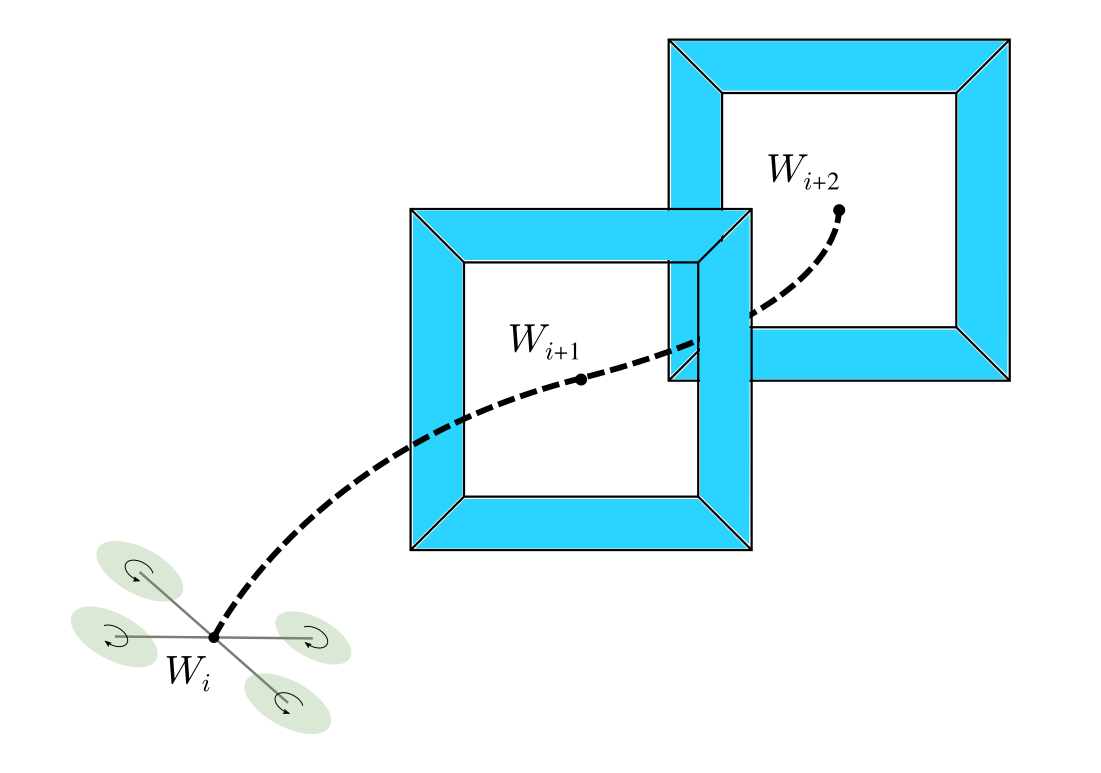
\includegraphics[width=0.7\textwidth]{imagenes/TrajCont}
	\caption{Esquema del objetivo de la generación de trayectorias empleando como waypoints los centros de las puertas y la posición del aeronave.}
	\label{TrajCont}
\end{figure}

Como se puede observar en el apartado anterior, las trayectorias que se generan entre dos puntos de paso $a$ y $b$, son trayectorias polinómicas cuyo grado depende del orden de la derivada de la acción de control. Debido a esto, se ha decidido usar trayectorias de tipo \textit{spline}, es decir, curvas diferenciables definidas en segmentos polinómicos, donde cada segmento sería una trayectoria entre dos \textit{waypoints}. Cada trayectoria completa, $r_d(t)$ está compuesta por $m$ segmentos de grado $q$, presentando la estructura

\begin{equation}
	r_d(t) = \left\{ 
	\begin{array}{ll}
		\sum_{i=0}^{q}a_{i1}t^{i} &,t_0\leq x \leq t_1 \\
		\sum_{i=0}^{q}a_{i2}t^{i} &,t_1\leq x \leq t_2 \\
		\qquad\vdots &\qquad\vdots \\
		\sum_{i=0}^{q}a_{im}t^{i} &,t_{m-1}\leq x \leq t_m \\
	\end{array}
	\right.
\end{equation}

siendo $a_{ij}\in \mathbb{R}$ los coeficientes de los polinomios. El grado $q$ de estos polinomios dependerá del índice a minimizar durante el transcurso de la trayectoria, como se ha explicado en el apartado \ref{trajectoriasoptimas:cap}. Cada tramo tiene un tiempo inicial y un tiempo final, estos tiempos dependen de las limitaciones físicas del aeronave, es decir, de su velocidad y aceleración máximas, en el apartado \ref{sec:estimacion_tiempos} se profundiza en la forma de generar estos tramos temporales.

De cara a resolver el valor de los distintos coeficientes de cada segmento polinomial se emplearán unas condiciones de contorno que garanticen la derivabilidad de la trayectoria completa en las $q$ primeras derivadas. 

Si se considera una trayectoria completa a través de $n$ \textit{waypoints} $P$ distribuidos a lo largo del tiempo, siendo $t_0$ el tiempo inicial del primer segmento y $t_n$ el tiempo final de la trayectoria, la trayectoria contará con $n-1$ segmentos polinómicos $S$ de grado $q$. Considerando que en el punto inicial y el punto final de la trayectoria el cuadricóptero se encuentra en un estado de equilibrio, las condiciones de contorno empleadas para calcular los coeficientes de la \textit{spline} son:
\begin{equation}
\begin{array}{ll}
	S_i (t = t_{i-1}) = W_{i-1} \quad &\forall i \in 1,...,n\\
	S_i (t = t_{i}) = W_i \quad &\forall i \in 1,...,n\\
	S_1^{(k)}(t = t_0) = 0 \quad &\forall k \in 1,...,q\\
	S_n^{(k)}(t = t_n) = 0 \quad &\forall k \in 1,...,q\\
	S_{i-1}^{(k)}(t = t_{i-1}) = S_{i}^{(k)}(t = t_{i})  \quad &\forall k \in 1,...,q \;; \forall n \in 2,...,n
\end{array}
\end{equation}
 siendo $W_i$ la posición del i-ésimo \textit{waypoint} , $S_i$ el i-ésimo segmento polinómico y  $t_i$ el tiempo de finalización del segmento $S_i$.
 
 Las dos primeras condiciones de contorno hacen referencia a las posiciones espaciales de los waypoints, es decir, que cada segmento empiece en un waypoint  y termine en el siguiente. Las dos condiciones siguientes hacen referencia al valor de las derivadas en los estados iniciales y final, se ha considerado que los estado inicial y final, son estados de equilibrio por lo que el valor de sus derivadas es nulo. Finalmente la ultima condición hace referencia a la continuidad de las derivadas entre segmentos, es decir, que el valor de las derivadas del final de un segmento, sean iguales al las derivadas iniciales del segmento siguiente, de esta forma se consigue que la trayectoria completa generada cumpla la condición de derivabilidad a lo largo de todas sus $q$ derivadas.

\section{Estimación de tiempos}\label{sec:estimacion_tiempos}

El objetivo final es generar trayectorias a través del circuito de forma que el aeronave sea capaz de recorrerlas teniendo en cuenta restricciones de posición, velocidad y aceleración. En los dos apartados anteriores se explica como generar trayectorias óptimas teniendo en cuentas restricciones de posición, fijando los \textit{waypoints} por los que se desea que pase el cuadricóptero. Sin embargo, para poder generar trayectorias es también necesario elegir los segmentos temporales $T_i$ entre los distintos puntos de paso, es decir, los tiempos que debe tardar el aeronave en pasar entre los distintos waypoints. Estos segmentos de tiempo deben tener en cuenta las limitaciones de velocidad y acceleración máximas del aeronave, para poder generar trayectorias realizables. A continuación se tratará un posible método para establecer la duración de estos intervalos temporales.

\subsubsection{Aproximación al tiempo medio}

La forma más sencilla de establecer intervalos temporales es basarse en la distancia existente entre un par de waypoints y la velocidad media a la que se desea que vuele el aeronave para estimar el tiempo necesario. Siendo $d_i = || W_{i-1} , W_{i} ||_2 $ la distancia entre dos \textit{waypoints} consecutivos y $v_m$ la velocidad media de vuelo, se puede establecer la duración de un segmento $S_i$ como
\begin{align}
	T_i = \frac{d_i}{v_m}
\end{align}
Para obtener los valores de tiempo absoluto $t_i$ requeridos en el apartado anterior simplemente se deben sumar las duraciones de los segmentos anteriores.
\begin{align}
t_i = \sum_{j=1}^{i} T_j
\end{align}


Para tener aumentar el control sobre la agresividad de la trayectoria se puede añadir un coeficiente $\alpha_i$ que permita modificar ligeramente el valor $T_i$ siendo 
\begin{align}
	T_i = \alpha_i\frac{d_i}{v_m}
\end{align}

Valores de $\alpha_i$ pequeños generan trayectorias más agresivas, así como valores más grandes producen trayectorias más seguras. Iterando el valor de este parámetro $\alpha_i$ se controla que las limitaciones en velocidad y aceleración máxima se cumplan para cada segmento $S_i$.

Esta es una forma simple y rápida de establecer los distintos segmentos temporales, sin embargo, es una aproximación que afecta a la generación de la trayectoria óptima, haciendo que el tiempo total que se tarda en recorrer el circuito sea mayor que el que se podría obtener usando otros métodos de optimización como los propuestos por Mellinger et al. \cite{MinimunSnap2011} o por Foehn. et al. \cite{foehn2020cpc}  para la obtención de estos segmentos temporales. A pesar de esto, debido a que las posiciones de los \textit{waypoints} cambian rápidamente a lo largo del circuito y se deben recalcular las trayectorias continuamente, el bajo coste computacional que presenta este método hace que merezca la pena su utilización.

